% ===================== AEGIS =====================
\subsection{AEGIS / Aegis-Bench}\label{ds:aegis}
\badgerow{\injected\ \okbadge\ \lbl{agent + failure mode (sets)}\ \lbl{MAS}\ \lbl{train / val / test}\ \lbl{MATH / GSM8K / HumanEval / SciBench / MMLU-Pro / GAIA}}

\begin{identity}
Paper & \emph{Aegis: Automated Error Generation and Attribution for Multi-Agent Systems} --- Kong, Zhang, Yin, Zhang, Zhang, Chen, Zhang, Zhang, Zhu, Feng (PKU, BIGAI, IIE CAS, NUS, Tsinghua), ICLR 2026, arXiv:2509.14295 \cite{aegis2026}\\
Links & \href{https://huggingface.co/datasets/Fancylalala/AEGIS}{HF \code{Fancylalala/AEGIS}} \textperiodcentered\ \href{https://github.com/kfq20/AEGIS}{GitHub \code{kfq20/AEGIS}} (injection factory, MAS wrappers, evaluation) \textperiodcentered\ \href{https://kfq20.github.io/AEGIS-Website/}{project page}\\
License & MIT (HF card and GitHub)\\
Status & downloaded in full, ungated; 222 MB; 9,533 trajectories = 600 test (\emph{Aegis-Bench}) + 7,146 train + 1,787 val; \code{data/attribution/aegis/}\\
\end{identity}

\paragraph{Description} AEGIS is the largest fully synthetic dataset in this survey, built for \emph{fine-grained error attribution}: given a failed MAS trajectory, predict the set of \textbf{(faulty agent, error mode)} pairs. It supports SFT, RL (GRPO with a hierarchical pair/agent/error reward) and contrastive learning on success/failure pairs; Aegis-Bench is the 600-trajectory test split (104--105 per non-GAIA benchmark and 76 GAIA). Construction:
\begin{itemize}
\item \textbf{Successful baselines} are run deterministically (all agents GPT-4o-mini per the paper, temperature 0; \code{metadata.model} is \code{unknown-model} on Magentic-One) for six MAS on MASLab---LLM Debate, MacNet (chain/star/tree/full topologies), AgentVerse, DyLAN, SmolAgents, Magentic-One---over MATH, GSM8K, HumanEval, SciBench, MMLU-Pro and GAIA (GAIA only for the last two systems; DyLAN has no MATH runs).
\item An LLM \textbf{adaptive manipulator} executes an injection plan, a set of (target agent, error modes), by \emph{prompt injection} (altering the agent's input) or \emph{response corruption} (replacing its output) through monkey-patched wrappers; corruptions are context-aware (plausible wrong arithmetic, infinite loops in code).
\item \textbf{Validation}: only runs whose final answer is wrong are kept; the injection plan becomes the label (refined post hoc for dynamic DyLAN graphs). Injection success: 76.5\% (Debate) down to 34.1\% (DyLAN).
\end{itemize}
\textbf{Taxonomy}: the 14 MAST failure modes---FM-1.1--1.5 specification issues (disobey task/role spec, step repetition, lost history, unaware of termination), FM-2.1--2.6 inter-agent misalignment (conversation reset, no clarification, derailment, withholding, ignored input, reasoning--action mismatch), FM-3.1--3.3 verification (premature termination, no/incorrect verification)---kept near-uniform by design (1,356--2,166 pairs each). \textbf{Quality check}: 100 Aegis-Bench trajectories blind-labelled by three experts, human--human Fleiss $\kappa$ = 0.85, programmatic-vs-human $\kappa$ = 0.81; MiniLM embeddings are interspersed with MAST-Data and Who\&When. \textbf{No step label}: the ground truth is agent + mode only; MacNet records add per-turn \code{is\_injected} flags on injected nodes, though in 1,210/2,359 MacNet trajectories \code{Node-2} is flagged while \code{faulty\_agents} collapses \code{Node-2} into \code{Node0}.

\paragraph{Metrics and baselines} Multi-label prediction of (agent, mode) pairs as JSON, scored by Micro-/Macro-F1 at three levels (Pair, Agent, Error); the paper averages 12 scores over Aegis-Bench and Who\&When (whose free-text reasons were mapped to FM modes by Gemini-2.5-Flash). Aegis-Bench, Micro-F1 in \% (paper):

\begin{center}\small
\begin{tabular}{@{}lccc@{}}\toprule
Model & Pair & Agent & Error\\\midrule
Random & 0.3 & 4.5 & 11.2\\
Qwen2.5-14B-Instruct & 5.5 & 35.8 & 20.2\\
GPT-4.1 & 7.4 & 37.5 & 20.7\\
o3 & 7.9 & 40.3 & 22.4\\
Gemini-2.5-Flash & 7.0 & 42.0 & 23.5\\
Claude-Sonnet-4 & 7.7 & 40.7 & 21.2\\
Aegis-SFT (Qwen2.5-14B) & \textbf{16.6} & \textbf{76.5} & \textbf{27.5}\\
Aegis-GRPO (Qwen2.5-14B) & 6.8 & 49.7 & 21.2\\
DCL (contrastive) & 8.3 & 22.9 & 24.7\\\bottomrule
\end{tabular}
\end{center}
Pair-level F1 is in single digits for every untuned model; SFT overfits the synthetic style after two epochs (Who\&When scores drop). Debate/AgentVerse are easier than DyLAN/MacNet.

\paragraph{Schema} \code{Aegis-Bench/test.jsonl}, \code{Aegis-Training/\allowbreak\{train,val\}.jsonl}, one object per line: \code{id} (\code{<Benchmark>\_<model>\_}\allowbreak\code{<framework>\_<idx>\_<hash>}), \code{metadata} (\code{framework}, \code{benchmark}, \code{model}, \code{task\_type}, \code{num\_agents}, \code{num\_injected\_agents}), \code{input.\allowbreak query}, \code{input.\allowbreak conversation\_history} (turns with 1-based \code{step}, \code{agent\_name}, \code{content} [null in 152 turns], \code{phase}; AgentVerse and DyLAN add \code{agent\_role} on subsets of turns, MacNet \code{is\_injected}), \code{input.\allowbreak final\_output} (present in 83.6\%; absent in all 1,567 DyLAN records), \code{output.faulty\_agents} = labels \{\code{agent\_name}, \code{error\_type}, \code{injection\_strategy}\}, \code{ground\_truth.correct\_answer}, \code{ground\_truth.injected\_agents} (same pairs plus \code{malicious\_action\_description}, empty in 68.1\% of pairs), \code{ground\_truth.is\_injection\_successful} (always true).

\paragraph{Statistics} computed from the downloaded JSONL.\par\nobreak\vspace{1pt}
\noindent\begin{minipage}[t]{0.54\linewidth}\vspace{0pt}\small
\fitbox{\begin{tabular}{@{}lrr@{}}\toprule
 & All & Test (Aegis-Bench)\\\midrule
trajectories (all failed, injected) & 9533 & 600\\
MATH / GSM8K / HumanEval & 2083 / 1778 / 1532 & 105 / 105 / 105\\
SciBench / MMLU-Pro / GAIA & 1905 / 1481 / 754 & 104 / 105 / 76\\
steps (turns): mean / median & 11.9 / 10 & 12.5 / 12\\
steps: min -- max & 3 -- 45 & 3 -- 43\\
distinct agents: mean (max) & 4.4 (8) & 4.3 (8)\\
(agent, mode) pairs / traj.: mean (max) & 2.38 (4) & 2.30 (4)\\
response corruption / prompt injection & 11964 / 10464 & 720 / 633\\
records with \code{is\_injected} markers & 24.8\% & 26.0\%\\
characters / traj.: mean & 20\,k & 21.5\,k\\\bottomrule
\end{tabular}}

\smallskip Per framework (all): AgentVerse 2,449, LLM Debate 2,404 (always 12 turns), MacNet 2,359 (10 turns; one 16-turn outlier), DyLAN 1,567, SmolAgents 481, Magentic-One 273; the two GAIA systems are longest (up to 45 turns; mean 45\,k--56\,k, max 285\,k chars vs.\ max 31\,k--66\,k for others). Blamed agents (unique traj.): Solver 2,281, Evaluator 1,934, RoleAssigner 1,752 (AgentVerse), Node0 2,000 (2,551 pairs incl.\ collapsed Node-2), Node3 1,815 (MacNet), Assistant1--3 (Debate/DyLAN), MagenticOneOrchestrator 129, WebSurfer 74. Where MacNet markers exist, the first injected turn sits at relative position 0.23 on average.
\end{minipage}\hfill
\begin{minipage}[t]{0.44\linewidth}\vspace{0pt}
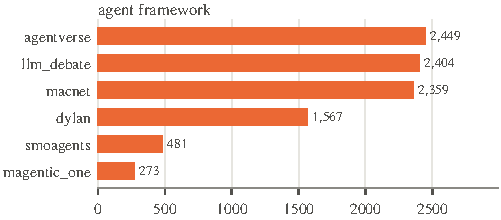
\includegraphics[width=\linewidth]{4_injected/aegis/figures/fw.pdf}
\end{minipage}

\paragraph{Example trajectory} \code{GSM8K\_gpt-4o-mini\_macnet\_12\_f7cdb106} (MacNet, 10 turns, 5 nodes, 8.4\,k characters), chosen because only MacNet records carry turn-level markers. Node1 is prompt-injected to repeat steps (FM-1.3) and Node3's responses are corrupted to terminate prematurely (FM-3.1); in Step~8 Node3 silently changes 10\%/20\% into 5\%/30\% (2.5 + 18 = 20.5, rounded to ``approximately 21''), which is retained as \code{final\_output} instead of 17 even though Node-2 corrects it to 17 in Steps~9--10. All five turns of the two injected nodes are marked.
% auto-generated by scripts/render_traj.py -- do not edit
\trajtask{GSM8K\_gpt-4o-mini\_macnet\_12\_f7cdb106}{Gabriel is looking at her marble sets. She sees that in the first set 10\% of her marbles are broken. In the second set,\allowbreak{} 20\% of the marbles are broken. The first set contains 50 marbles. The second set contains 60. How many marbles are broken in total?\allowbreak{}}
\begin{trajstep}{1}{Node-1}{agA}
To determine the total number of broken marbles in Gabriel's sets,\allowbreak{} follow these steps:\allowbreak{}\par 1. **Identify the number of marbles in each set:\allowbreak{}**\newline - **First Set:\allowbreak{}** 50 marbles\newline - **Second Set:\allowbreak{}** 60 marbles\par 2. **Calculate the number of broken marbles in each set:\allowbreak{}**\newline - **First Set:\allowbreak{}**\newline - Percentage broken:\allowbreak{} 10\%\newline - Calculation:\allowbreak{} \textbackslash{}( 10\textbackslash{}\% \textbackslash{}text\{ of \} 50 =\allowbreak{} 0.10 \textbackslash{}times 50 =\allowbreak{} 5 \textbackslash{}) broken marbles\par - **Second Set:\allowbreak{}**\newline - Percentage broken:\allowbreak{} 20\%\newline - Calculation:\allowbreak{} \textbackslash{}( 20\textbackslash{}\% \textbackslash{}text\{ of \} 60 =\allowbreak{} 0.20 \textbackslash{}times 60 =\allowbreak{} 12 \textbackslash{}) broken marbles\par 3. **Add the broken marbles from both sets:\allowbreak{}**\newline - Total broken marbles:\allowbreak{} \textbackslash{}( 5 \textbackslash{}text\{ (from the first set)\} + 12 \textbackslash{}text\{ (from the second set)\} =\allowbreak{} 17 \textbackslash{})\par 4. **Final Answer:\allowbreak{}**\newline - The total number of broken marbles in both sets is **17**.
\end{trajstep}
\begin{trajstep}{2}{Node0}{agB}
<INFO>No revision needed
\end{trajstep}
\begin{trajstep}{3}{Node0}{agB}
To find the total number of broken marbles in Gabriel's sets,\allowbreak{} follow these steps:\allowbreak{}\par 1. **Identify the Number of Marbles:\allowbreak{}**\newline - **First Set:\allowbreak{}** 50 marbles\newline - **Second Set:\allowbreak{}** 60 marbles\par 2. **Calculate Broken Marbles in Each Set:\allowbreak{}**\newline - **First Set (10\% broken):\allowbreak{}**\newline - Calculation:\allowbreak{} \textbackslash{}( 10\textbackslash{}\% \textbackslash{}times 50 =\allowbreak{} 0.10 \textbackslash{}times 50 =\allowbreak{} 5 \textbackslash{}) broken marbles\newline - **Second Set (20\% broken):\allowbreak{}**\newline - Calculation:\allowbreak{} \textbackslash{}( 20\textbackslash{}\% \textbackslash{}times 60 =\allowbreak{} 0.20 \textbackslash{}times 60 =\allowbreak{} 12 \textbackslash{}) broken marbles\par 3. **Total Broken Marbles:\allowbreak{}**\newline - Total:\allowbreak{} \textbackslash{}( 5 \textbackslash{}text\{ (from the first set)\} + 12 \textbackslash{}text\{ (from the second set)\} =\allowbreak{} 17 \textbackslash{})\par 4. **Final Answer:\allowbreak{}**\newline - The total number of broken marbles in both sets is **17**.
\end{trajstep}
\begin{faultystep}{4}{Node1}{agC}
The answer provided is generally accurate and covers the necessary calculations,\allowbreak{} but it has some areas that could be improved for clarity and conciseness.\par 1. **Accuracy**:\allowbreak{} The calculations for the number of broken marbles in each set are correct. 5 broken marbles in the first set and 12 in the second set,\allowbreak{} totaling 17 broken marbles.\par 2. **Completeness**:\allowbreak{} The answer covers all aspects of the user's question by detailing the number of marbles in each set,\allowbreak{} the percentage of broken marbles,\allowbreak{} and the final total.\par 3. **Logical**:\allowbreak{} The organization is somewhat repetitive,\allowbreak{} particularly in the verification and confirmation steps. While it is import\newline [...] (1,\allowbreak{}074 chars omitted) [...]\newline times 60 =\allowbreak{} 12 \textbackslash{}) broken marbles\par 3. **Total Broken Marbles:\allowbreak{}**\newline - Total:\allowbreak{} \textbackslash{}( 5 + 12 =\allowbreak{} 17 \textbackslash{})\par The total number of broken marbles in both sets is **17**.\par ---\par This revision maintains accuracy and completeness while improving logical flow and relevance.
\end{faultystep}
\begin{faultystep}{5}{Node1}{agC}
To optimize the answer based on review suggestions,\allowbreak{} we can streamline the explanation,\allowbreak{} reduce repetition,\allowbreak{} and maintain clarity. Here's the revised response:\allowbreak{}\par ---\par To determine the total number of broken marbles in Gabriel's sets,\allowbreak{} we can follow these steps:\allowbreak{}\par 1. **Identify the Number of Marbles:\allowbreak{}**\newline - **First Set:\allowbreak{}** 50 marbles\newline - **Second Set:\allowbreak{}** 60 marbles\par 2. **Calculate Broken Marbles in Each Set:\allowbreak{}**\newline - **First Set (10\% broken):\allowbreak{}**\newline - Calculation:\allowbreak{} \textbackslash{}( 10\textbackslash{}\% \textbackslash{}times 50 =\allowbreak{} 0.10 \textbackslash{}times 50 =\allowbreak{} 5 \textbackslash{}) broken marbles\newline - **Second Set (20\% broken):\allowbreak{}**\newline - Calculation:\allowbreak{} \textbackslash{}( 20\textbackslash{}\% \textbackslash{}times 60 =\allowbreak{} 0.20 \textbackslash{}times 60 =\allowbreak{} 12 \textbackslash{}) broken marbles\par 3. **Total Broken M\newline [...] (69 chars omitted) [...]\newline from the second set)\} =\allowbreak{} 17 \textbackslash{})\par 4. **Final Answer:\allowbreak{}**\newline - The total number of broken marbles in both sets is **17**.\par ---\par This version maintains the essential calculations while eliminating unnecessary repetitions and providing a clear,\allowbreak{} concise answer.
\end{faultystep}
\begin{faultystep}{6}{Node3}{agD}
To determine the total number of broken marbles in Gabriel's sets,\allowbreak{} we can follow these steps:\allowbreak{}\par 1. **Identify the Number of Marbles:\allowbreak{}**\newline - **First Set:\allowbreak{}** 50 marbles\newline - **Second Set:\allowbreak{}** 60 marbles\par 2. **Calculate Broken Marbles in Each Set:\allowbreak{}**\newline - **First Set (10\% broken):\allowbreak{}**\newline - Calculation:\allowbreak{} \textbackslash{}( 10\textbackslash{}\% \textbackslash{}times 50 =\allowbreak{} 0.10 \textbackslash{}times 50 =\allowbreak{} 10 \textbackslash{}) broken marbles\newline - **Second Set (20\% broken):\allowbreak{}**\newline - Calculation:\allowbreak{} \textbackslash{}( 20\textbackslash{}\% \textbackslash{}times 60 =\allowbreak{} 0.20 \textbackslash{}times 60 =\allowbreak{} 15 \textbackslash{}) broken marbles\par 3. **Total Broken Marbles:\allowbreak{}**\newline - Total:\allowbreak{} \textbackslash{}( 10 \textbackslash{}text\{ (from the first set)\} + 15 \textbackslash{}text\{ (from the second set)\} =\allowbreak{} 25 \textbackslash{})\par 4. **Final Answer:\allowbreak{}**\newline - The total number of broken marbles in both sets is **25**.
\end{faultystep}
\begin{faultystep}{7}{Node3}{agD}
The answer provided seems to have several inaccuracies that could lead to confusion. It incorrectly calculates the number of broken marbles in both sets and fails to sum them up correctly,\allowbreak{} resulting in an erroneous final answer.\par There are also critical oversights in the methodology,\allowbreak{} as it combines unrelated data points which are irrelevant to the analysis of the marbles. This could mislead users into thinking that the calculations are accurate when they are not.\par **Area for Improvement:\allowbreak{}**\newline - **Logical Errors:\allowbreak{}** The calculations need to be re-evaluated as they don't add up based on the data presented.\par **Specific Suggestions for Revision:\allowbreak{}**\newline [...] (253 chars omitted) [...]\newline y.\par Overall,\allowbreak{} while the answer is presented in a structured manner,\allowbreak{} the redundancy and flawed calculations contribute to a lack of clarity that could mislead users.\par Final recommendation:\allowbreak{}\newline <INFO>Further analysis is required to clarify the discrepancies.
\end{faultystep}
\begin{faultystep}{8}{Node3}{agD}
To determine the total number of broken marbles in Gabriel's sets,\allowbreak{} follow these steps:\allowbreak{}\par 1. **Identify the Number of Marbles:\allowbreak{}**\newline - **First Set:\allowbreak{}** 50 marbles\newline - **Second Set:\allowbreak{}** 60 marbles\par 2. **Calculate Broken Marbles in Each Set:\allowbreak{}**\newline - **First Set (5\% broken):\allowbreak{}**\newline - Calculation:\allowbreak{} \textbackslash{}( 5\textbackslash{}\% \textbackslash{}times 50 =\allowbreak{} 0.05 \textbackslash{}times 50 =\allowbreak{} 2.5 \textbackslash{}) broken marbles\newline - **Second Set (30\% broken):\allowbreak{}**\newline - Calculation:\allowbreak{} \textbackslash{}( 30\textbackslash{}\% \textbackslash{}times 60 =\allowbreak{} 0.30 \textbackslash{}times 60 =\allowbreak{} 18 \textbackslash{}) broken marbles\par 3. **Total Broken Marbles:\allowbreak{}**\newline - Total:\allowbreak{} \textbackslash{}( 2.5 \textbackslash{}text\{ (from the first set)\} + 18 \textbackslash{}text\{ (from the second set)\} =\allowbreak{} 20.5 \textbackslash{})\par 4. **Final Answer:\allowbreak{}**\newline - The total number of broken marbles in both sets is approximately **21**.
\end{faultystep}
\begin{trajstep}{9}{Node-2}{agE}
The area that needs the most improvement is **accuracy**.\par Specific suggestions for revision:\allowbreak{}\par 1. **Correct the Percentage Calculations:\allowbreak{}**\newline - The first set has 10\% broken marbles,\allowbreak{} not 5\%. The calculation should be:\allowbreak{}\newline - **First Set:\allowbreak{}** \textbackslash{}( 10\textbackslash{}\% \textbackslash{}times 50 =\allowbreak{} 0.10 \textbackslash{}times 50 =\allowbreak{} 5 \textbackslash{}) broken marbles.\newline - The second set has 20\% broken marbles,\allowbreak{} not 30\%. The calculation should be:\allowbreak{}\newline - **Second Set:\allowbreak{}** \textbackslash{}( 20\textbackslash{}\% \textbackslash{}times 60 =\allowbreak{} 0.20 \textbackslash{}times 60 =\allowbreak{} 12 \textbackslash{}) broken marbles.\par 2. **Update the Total Calculation:\allowbreak{}**\newline - The total broken marbles should be:\allowbreak{}\newline - Total:\allowbreak{} \textbackslash{}( 5 \textbackslash{}text\{ (from the first set)\} + 12 \textbackslash{}text\{ (from the second set)\} =\allowbreak{} 17 \textbackslash{}).\par 3. **Revise the Final Answer:\allowbreak{}**\newline - The final answer should state that the total number of broken marbles in both sets is **17**.\par By addressing these inaccuracies,\allowbreak{} the answer will be correct and meet the review criteria more effectively.
\end{trajstep}
\begin{trajstep}{10}{Node-2}{agE}
To determine the total number of broken marbles in Gabriel's sets,\allowbreak{} follow these steps:\allowbreak{}\par 1. **Identify the Number of Marbles:\allowbreak{}**\newline - **First Set:\allowbreak{}** 50 marbles\newline - **Second Set:\allowbreak{}** 60 marbles\par 2. **Calculate Broken Marbles in Each Set:\allowbreak{}**\newline - **First Set (10\% broken):\allowbreak{}**\newline - Calculation:\allowbreak{} \textbackslash{}( 10\textbackslash{}\% \textbackslash{}times 50 =\allowbreak{} 0.10 \textbackslash{}times 50 =\allowbreak{} 5 \textbackslash{}) broken marbles\newline - **Second Set (20\% broken):\allowbreak{}**\newline - Calculation:\allowbreak{} \textbackslash{}( 20\textbackslash{}\% \textbackslash{}times 60 =\allowbreak{} 0.20 \textbackslash{}times 60 =\allowbreak{} 12 \textbackslash{}) broken marbles\par 3. **Total Broken Marbles:\allowbreak{}**\newline - Total:\allowbreak{} \textbackslash{}( 5 \textbackslash{}text\{ (from the first set)\} + 12 \textbackslash{}text\{ (from the second set)\} =\allowbreak{} 17 \textbackslash{})\par 4. **Final Answer:\allowbreak{}**\newline - The total number of broken marbles in both sets is **17**.
\end{trajstep}
\trajannotation{['Node1',\allowbreak{} 'Node3']}{4,\allowbreak{} 5,\allowbreak{} 6,\allowbreak{} 7,\allowbreak{} 8}{["FM-1.3",\allowbreak{} "FM-3.1"]}{Node 1 injected with prompt\_injection;\allowbreak{} Node 3 injected with response\_corruption}{In the first set there are 5 broken marbles because 50 x .1 =\allowbreak{} <<50*.1=\allowbreak{}5>>5\newline In the second set there are 12 broken marbles because 60 x .2 =\allowbreak{} <<60*.2=\allowbreak{}12>>12\newline There are 17 broken marbles in total because 5 + 12 =\allowbreak{} <<5+12=\allowbreak{}17>>17\newline \#\#\#\# 17}{To determine the total number of broken marbles in Gabriel's sets,\allowbreak{} follow these steps:\allowbreak{}\par 1. **Identify the Number of Marbles:\allowbreak{}**\newline - **First Set:\allowbreak{}** 50 marbles\newline - **Second Set:\allowbreak{}** 60 marbl\newline [...] (420 chars omitted) [...]\newline The total number of broken marbles in both sets is approximately **21**.}{\textbf{faulty\_agents\_pairs}: [\{"agent\_name":\allowbreak{} "Node1",\allowbreak{} "error\_type":\allowbreak{} "FM-1.3",\allowbreak{} "injection\_strategy":\allowbreak{} "prompt\_injection"\},\allowbreak{} \{"agent\_name":\allowbreak{} "Node3",\allowbreak{} "error\_type":\allowbreak{} "FM-3.1",\allowbreak{} "injection\_strategy":\allowbreak{} "response\_corruption"\}]; \textbf{injected\_agents}: [\{"agent\_name":\allowbreak{} "Node1",\allowbreak{} "error\_type":\allowbreak{} "FM-1.3",\allowbreak{} "injection\_strategy":\allowbreak{} "prompt\_injection",\allowbreak{} "malicious\_action\_description":\allowbreak{} "Node 1 injected with prompt\_injection"\},\allowbreak{} \{"agent\_name":\allowbreak{} "Node3",\allowbreak{} "error\_type":\allowbreak{} "FM-3.1",\allowbreak{} "injection\_strategy":\allowbreak{} "response\_corruption",\allowbreak{} "malicious\_action\_description":\allowbreak{} "Node 3 injected with response\_corruption"\}]; \textbf{injection\_strategies}: ["prompt\_injection",\allowbreak{} "response\_corruption"]; \textbf{metadata}: \{"framework":\allowbreak{} "macnet",\allowbreak{} "benchmark":\allowbreak{} "GSM8K",\allowbreak{} "model":\allowbreak{} "gpt-4o-mini",\allowbreak{} "num\_agents":\allowbreak{} 5,\allowbreak{} "num\_injected\_agents":\allowbreak{} 2,\allowbreak{} "task\_type":\allowbreak{} "math"\}; \textbf{is\_injection\_successful}: True; \textbf{step\_indexing}: 1-based field conversation\_history[].step; \textbf{note}: AEGIS labels are agent+error-mode level;\allowbreak{} step-level label only via is\_injected markers where present}


\paragraph{Notes} (i) The only dataset here whose primary label is a \emph{set} of (agent, mode) pairs (mean 2.4, up to 4); no decisive step is annotated, so step-level attribution cannot be evaluated on AEGIS (MacNet's \code{is\_injected} flags every turn of an injected node rather than one step, and disagrees with \code{faulty\_agents} in 51.3\% of MacNet runs due to \code{Node-2}$\to$\code{Node0} collapse). (ii) Failures are fully synthetic, injected into GPT-4o-mini runs and shaped after MAST modes rather than naturally occurring slips; realism rests on $\kappa$ = 0.81 and embedding overlap. (iii) Short, homogeneous trajectories (median 10 turns, $\approx$5\,k tokens) with structural agent names. (iv) Data/paper discrepancies: per-framework and per-benchmark counts differ from the paper's Table 2 (e.g.\ AgentVerse 2,449 vs 1,995, Magentic-One 273 vs 449), pair total 22,701 vs 24,843; naming quirks \code{smoagents}, \code{magentic+gaia}, \code{smol+gaia}, \code{MMLU} (for MMLU-Pro), and \code{unknown-model} on Magentic-One; a third strategy value \code{prompt} (273 pairs); \code{num\_injected\_agents} $\ne$ number of pairs in 22\% of records; two IDs duplicated across train and val with identical labels but distinct histories. (v) Shares Magentic-One/SmolAgents + GAIA with Who\&When, MAST and TracerTraj (shared author), but all runs are the authors' own; VerifyMAS (2026) reuses Aegis-Bench with a global/local/hybrid grouping of the modes. (vi) MIT licence and modest size make it the most convenient large training set in this survey.
